%% This is an example first chapter.  You should put chapter/appendix that you
%% write into a separate file, and add a line \include{yourfilename} to
%% main.tex, where `yourfilename.tex' is the name of the chapter/appendix file.
%% You can process specific files by typing their names in at the 
%% \files=
%% prompt when you run the file main.tex through LaTeX.
\chapter{Docker Fundamentals}
\label{chap:docker}

Docker is a relatively new open-source framework that serves as a lightweight alternative to virtual machines. It provides users with the ability to create isolated, high-performing containers that can be seamlessly deployed to other hosts that are also running the Docker Engine. Unlike virtual machines, containers share the kernel with the host and therefore rely on specific features in the kernel to provide a comparable level of isolation. For now, these containers are restricted to Linux; however, Microsoft has recently made a commitment to bring container technology based on Docker to the Windows platform \cite{windows-docker}.

For the past few years, Docker has been under active heavy development and in recent months is gaining popularity across the industry. An extraordinary number of new projects and platforms are being built on top of Docker, resulting in a rich and lively ecosystem. 


In section~\ref{ch2:system}, we outline the technical details of Docker; in section~\ref{ch2:lingo}, we describe fundamental terms that will be essential to the understanding of VM2Docker; in section~\ref{ch2:usecase} we dive into the wide variety of use cases Docker containers can have; and finally in section~\ref{ch2:industry} we discuss the industry's response to Docker.

\section{System Details}\label{ch2:system}
The Docker platform is divided into the Docker Engine, which supports the runtime and execution of containers, and the Docker Registry, which provides the hosting and delivery of a repository of Docker images. Each container provides a namespaced, isolated environment for execution. Docker exploits filesystem layering, as well as specific features of the Linux kernel to make all of these possible.

\begin{figure}[h]
\centering
    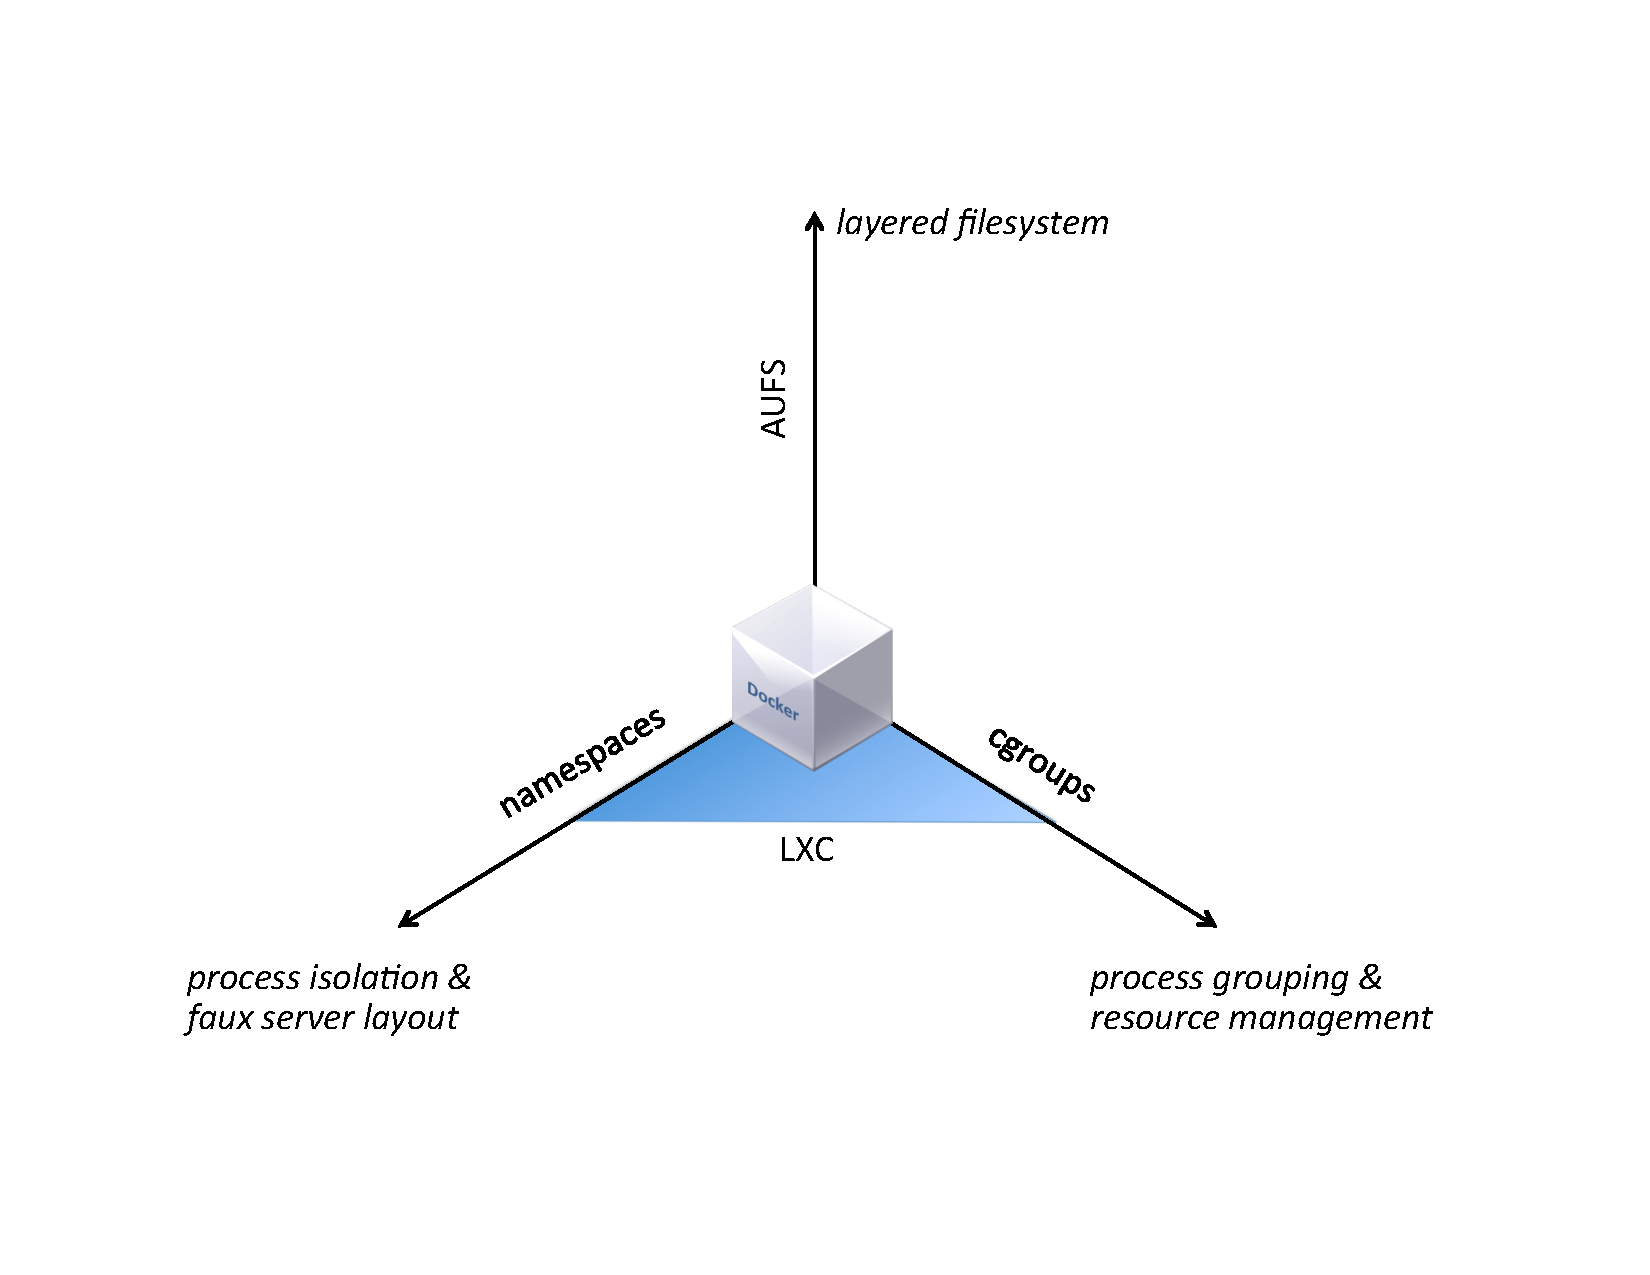
\includegraphics[width=1.0\textwidth]{docker.pdf}
    \caption{A graphic outlining the three fundamental components that make up the Docker framework. Namespace and cgroup support are provided by the LXC (LinuX Container) kernel extensions, and filesystem layering is provided by AUFS.}
\end{figure}

\subsection{cgroups}
Cgroups, or control groups, are a feature on the Linux kernel that provides resource limiting, in the form of memory or disk limits, as well as prioritization of CPU and disk throughput. These features are comparable to those offered by a virtual machine hypervisor to allocate a given amount of memory and CPU, network, and disk priority to a virtual machine.

\subsection{namespaces}

Namespaces are the mechanism by which each Docker container is isolated from the host and other containers. There are many different namespaces that LXC supports, but perhaps the two most significant ones are the \texttt{pid} and \texttt{net} namespaces. The \texttt{pid} namespace is responsible for giving each container its own isolated environment for processes. A given container can only see and send signals to the processes that are running within the same container. In addition, the \texttt{net} namespace allows different containers to have what appears to be distinct network interfaces, thereby permitting two containers to simultaneously bind to the same port, for example \cite{lxc}.

\subsection{Another Union FileSystem (AUFS)}
AUFS, Another Union FileSystem, is the primary means through which Docker achieves both storage savings and faster deployments of containers. Each image inherits from a sequence of other images, up to the base image, and represents the set or sequence of changes on the filesystem. This layering of filesystems and images accomplishes two main benefits. First, it allows for a high degree of storage savings. If two containers are running the same OS and share some libraries and dependencies, the majority of their filesystems will only be represented once on disk and are not duplicated. Second, when downloading and deploying a container, if a host already has previous layers of the filesystem on which a given container depends, it need only download the incremental changes.

\subsection{Docker Registry}
Docker provides a public registry to which developers can push their custom Docker images and share their creations with others \cite{dockerregistry}. It has support for creating private images, but requires the user to pay to have more than one privately hosted image.

Docker also has open sourced the Docker Registry \cite{dockerregistry-github} to allow for privately hosted registries. For enterprises, this is a superior solution that allows for easy deployment and configuration of Docker containers across a wide area datacenter.

\section{Technical Terms}\label{ch2:lingo}
The comprehension of a few terms related to Docker is essential to the understanding of this thesis. 
\subsection{Dockerfile}
A Dockerfile, similar to a Makefile, is composed of a set of instructions used by Docker to build an image. It typically starts with an inheritance line, specifying from which image to inherit. This can either be a base image, or another image that has been previously built. After the inheritance instruction, the rest of the Dockerfile consists of a combination of commands to run, files to add, environment variables to set, and ports to expose. The Dockerfile can then be passed into the Docker engine, along with an optional tag, and the resulting image is built. Each command in the Dockerfile represents a new layer on the file system. Each change is performed, copy-on-write, such that the entire image ancestry is accessible at any time.

\subsection{Base Image}
A base image is a special kind of Docker image that does not have a parent image. The base image instead represents the set of files that make a given operating system unique, excluding the kernel. Examples of base images are Ubuntu 14.04 and CentOS7. Base images do not have a parent and instead fully represent an entire OS on their own. Base images are used as starting points from which all other images can inherit \cite{baseimage}. 

\subsection{Containers vs. Images}
Images are read-only layers on the filesystem. Each layer is a distinct image. To run a container, one specifies an image and a command to run. All changes to the filesystem go to the top-most container layer of the filesystem, preserving all image layers beneath. Figure~\ref{ch2:imagevcontainers} illustrates all of these concepts.

\begin{figure}[h]
\centering
    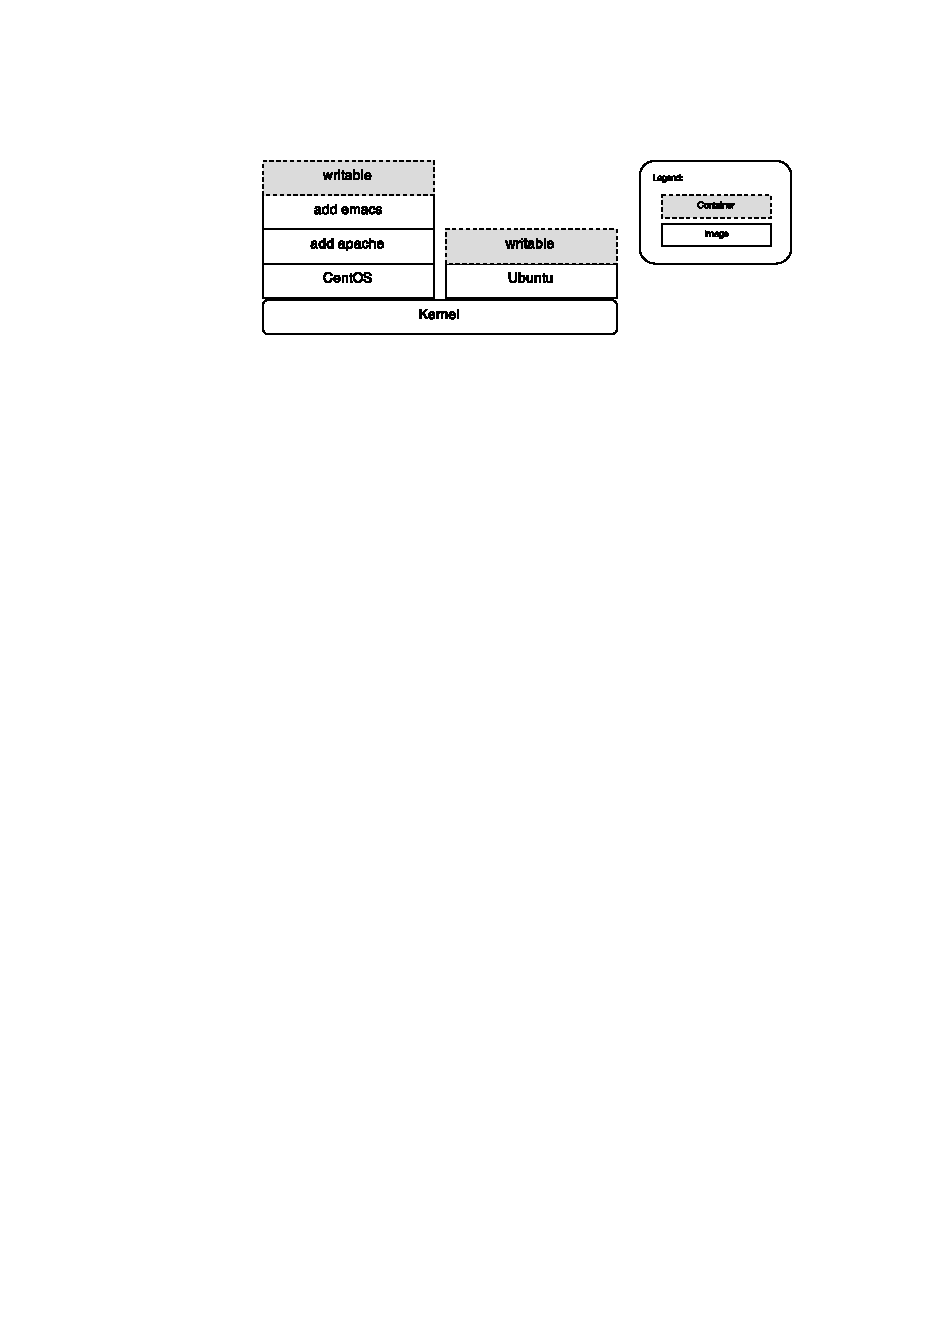
\includegraphics[width=1.0\textwidth]{cvimage.pdf}
    \caption{A graphic providing examples of the difference between containers and images in the Docker Engine. Containers are the top-most writable layers of the filesystem and represented by the rectangles with dashed lines and grey background. Images are the read-only layers used for inheritance and are represented by the rectangles with the solid lines and white background.}
\label{ch2:imagevcontainers}
\end{figure}

\section{Use Cases}\label{ch2:usecase}
\subsection{Cloud}
This is the primary target for which VM2Docker is geared. As an alternative to hosting virtual machines in the cloud, many cloud providers now offer the option to either directly use containers, run containers within a container-optimized VM, or both.

\subsection{DevOps}
Another essential audience for the Docker framework is the DevOps paradigm. DevOps is the process by which a piece of software is developed and subsequently deployed, along with the continuous revision process of simultaneous development and deployment. Historically, DevOps has been challenging to get right because of all of the dependencies a certain piece of software might have. During deployment, the software installed on a given developer's host must also be installed on the host running the deployed application. Docker provides a streamlined way to guarantee that a piece of software running on one host will run exactly the same on another host, as long as each host has the Docker Engine installed. This guarantee is an invaluable asset and is touted as the "first true" DevOps tool \cite{devops}. Ops managers may choose to deploy the Docker containers in the cloud or in their own private cluster of Docker-supported machines.

%\subsection{Benefits \& Drawbacks}\label{ch2:bd}
%https://news.ycombinator.com/item?id=8167928

\section{Industry Hype}\label{ch2:industry}

The hype over Docker, both in the open-source community as well as in the industry, has been unprecedented. In the past year and even more recently in the past six months, a number of influential players in the cloud hosting industry have begun to offer native support for running Docker containers. Specifically, Amazon has launched its own EC2 container service \cite{aws} and Google has their own container engine powered by the open-source cluster manager Kubernetes, Additionally, VMware, initially perceived to be threatened by container technology, has announced a partnership with Docker which attempts improve the overall user experience \cite{vmware}. In addition to the established cloud providers, other providers such as Tutum and Orchard, which was acquired by Docker, have been created that focus specifically on container deployment in the cloud. The excitement and popularity of the Docker framework across the industry is a testament to its utility and novelty as compared to the prior industry standard, virtual machines.

\subsection{Comparison to Virtual Machines}
While it remains to be seen whether Docker poses an immediate threat to the virtual machine landscape, it is evident that virtual machines and containers are distinct products that aren't necessarily direct competitors. Each caters to a slightly different audience.

Since Docker shares the kernel with the host, it only supports Linux-based containers and immediately discards support for legacy enterprise software that might need a Windows environment to run.

Central to the distinction between container and virtual machine is the tradeoff between density and isolation. Virtual machines offer the strongest form of isolation, comparable to that offered by physically separated hosts. Containers, on the other hand, share the kernel with the host, and therefore provide a much larger attack surface through which an attacker might be able to compromise another container on the same host. 

By giving up isolation, unlike virtual machines which incur a performance overhead, containers achieve near native performance as compared to running directly on the host itself \cite{performance}. Furthermore, the density of containers on a given host can be much higher than that of VMs. 

\begin{figure}[h]
\centering
\subfigure[Docker Container]{%
  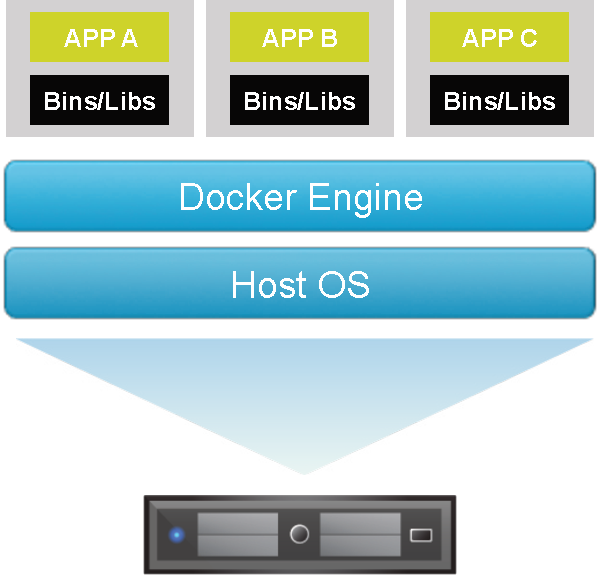
\includegraphics[width=.4\linewidth]{docker_h.pdf}
  \label{fig:sub1}}
\quad
\quad
\subfigure[Virtual Machine]{%
  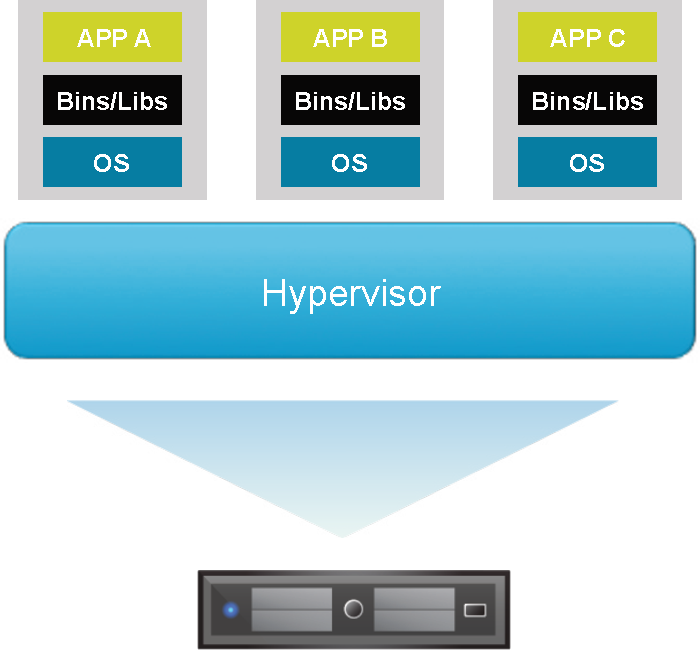
\includegraphics[width=.4\linewidth]{vm_h.pdf}
  \label{fig:sub2}}
\caption{A comparison of the components and isolation of virtual machines as compared to Docker containers. Each container consists of only an application and its dependencies and shares the underlying kernel with the host OS.}
\label{fig:test}
\end{figure}

Since Docker can run directly inside of a virtual machine, but not vice versa, there are interesting ways in which Docker and VMware VMs might be able to work together in the future to offer a streamlined experience that captures the benefits of each. Multiple, trusted, containers running in the same VM, for example, could provide stronger isolation while still achieving the portability and deployment benefits that Docker containers provide.

Another distinct advantage of VMs is there ability to perform live migrations from one host to another. VMware dubs this process vMotion\cite{vmotion}, and it is used as a direct building block for VMware's Dynamic Resource Scheduling (DRS)\cite{DRS}. Docker containers, unless running in a VM (and migrated with vMotion), cannot be live migrated to another host and instead must be shut down, moved, and started back up. CRIU\cite{CRIU} is a project under heavy active active development that attempts to bring this live migration to the container ecosystem by implementing checkpoint/restore functionality for Linux in userspace. Once completed, CRIU might be used as a primitive for dynamic resource scheduling among different Docker host. However, as of this writing, no such feature exists.
\subsection{Competitors}
Docker is one of the most successful and popular frameworks for container technology. However, there are also a number of other alternatives that are also built on top of Linux containers. 

\subsubsection{Flockport}
Flockport is a young alternative to Docker that focuses on entire virtualization workloads, instead of app delivery. As a result, Flockport does not boast the same kind of layered filesystem as Docker and instead is built on top of the LXC protocol \cite{flockport}.

\subsubsection{Spoonium}
Spoonium is a platform that attempts to bring container technologies to platforms not necessarily based on Linux. It touts many of the features of the Docker framework. Interestingly, Docker, too, has announced its intention of bringing Docker support to the Windows platform. Thus, it remains to be seen of Spoonium will experience the same kind of success that Docker has.

\subsubsection{Rocket - CoreOS}
Rocket, by CoreOS, is an alternative to Docker under heavy active development. CoreOS initially provided complete support for Docker, and their operating system was specifically built as a bare-bones operating system with the minimal amount of software installed to run Docker. A variety of disputes over the overall product vision has inspired CoreOS to develop their own take on containers, called Rocket, and we will see what sort of improvements and following this gets in the coming months and the software matures \cite{rocket}.

\subsubsection{Ubuntu - LXD}
One final player in the container field is Ubuntu and their announcement of LXD. LXD aims to build on top of LXC and serve as a hypervisor for containers. A main feature it aims to support is the live snapshotting of containers through CRIU\cite{CRIU}, which also enables them to support live migration of containers between hosts. These features are invaluable and would serve as an essential addition to the container framework, thereby bringing some of this container technology inline with that offered by VMware and vMotion and DRS \cite{vmotion,DRS}. Since LXD will work on a slightly lower level of the stack than Docker, it is possible it will also serve as an enhancement, rather than a direct competitor, to Docker \cite{lxd}.

%\subsection{Orchestration}




